With the structure of the components defined, the model and function components will now be analysed further.

\subsubsection{Model Component}
\label{ModelComponentSec}

The model component only contains the the DB component, as seen in Figure \ref{Components}. What is included here is the original class structure, which is now going to be inserted into the model layer as its components, after it has been updated. This update is based on the event table which was created in the problem area analysis, and with implementation in mind. See section \ref{ProblemDomain}

Following the theory, the class diagram has been updated to become the model component, taking into consideration private and shared events, and whether or they are iterative or singular. For example, the add/remove friend events become a class for itself, called the friends list, and is a part of the class it had a singular iterative connection with, which was the media interested person class. The other add/remove event for media had a shared iterative connection, so it is more open how this is can be shown on the new class diagram. In Figure \ref{ModelComponent} you can see it as a new layer between the media interested person and the media classes, and is called the medialist.

\begin{figure}[htb]
\centering
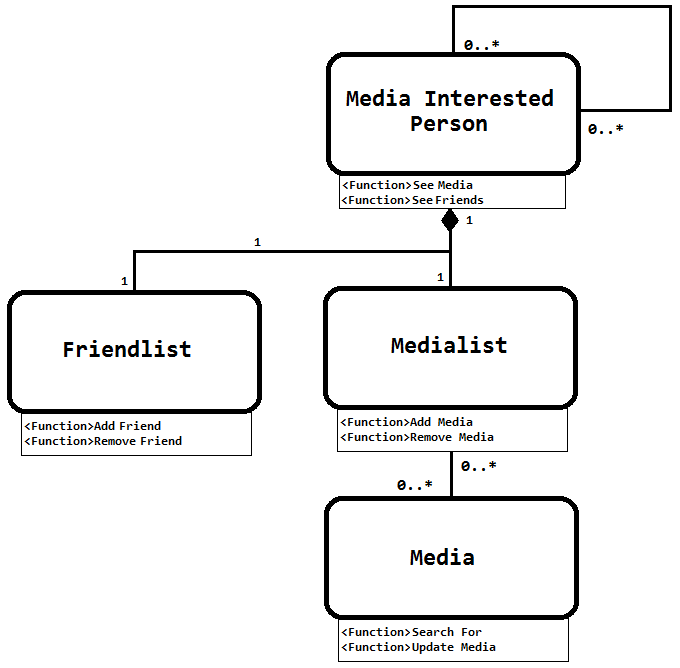
\includegraphics[width=0.7\textwidth]{Images/modelcomponent.png}
\caption{The model component with associated functions}
\label{ModelComponent}
\end{figure}

\subsubsection{Function Component}

The function component is made by going back to the functions that was defined in a previous section and adding them to the updated component diagram. See Figure \ref{FullComponents}. Their placement is dependent on how many classes have relations to the specific functions. If a function only affects one type of class, the function can be added directly to the class inside the model component. This can be seen in Figure \ref{ModelComponent}. If it affects several, then it should be a separate component inside the function component, pointing to the classes in the model component on which it has an effect.

For example, the ‘Generate Recommendations’ function, works not only on media in the system, but also on users, for which it generates media recommendations. It was already defined in the function component and this confirms its position there. The add/remove media and friends functions is limited to only one kind of class, and it is therefore attached to that class in the model component.

\begin{figure}[htb]
\centering
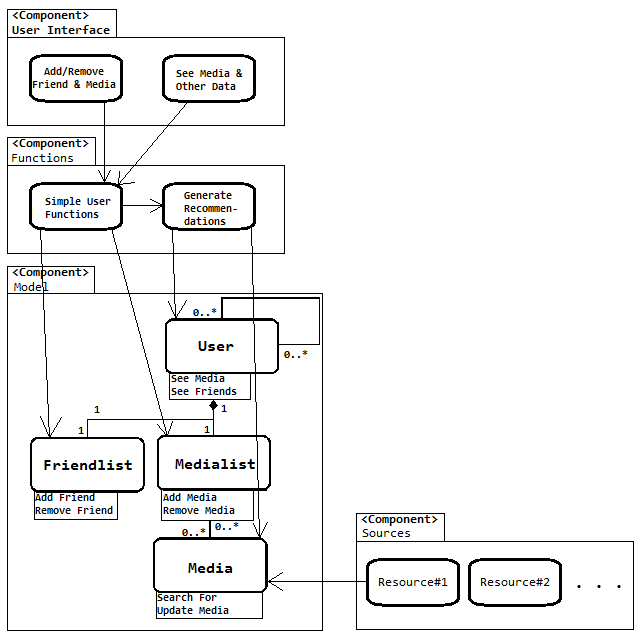
\includegraphics[width=0.7\textwidth]{Images/FullComponents.png}
\caption{The full component structure}
\label{FullComponents}
\end{figure}